\documentclass[14pt,a4paper,oneside]{article}

\usepackage[utf8]{inputenc}   


\usepackage{amsmath,amsthm,amssymb,appendix,bm,mathrsfs,ctex,geometry,tcolorbox,fancyhdr,tikz,esint,appendix}


%% GB/T 7714 宏包 ---- 引文格式
\usepackage[sort&compress]{gbt7714}
\bibliographystyle{gbt7714-numerical}



% \numberwithin{equation}{section}             %%%%%% 公式编号




\geometry{left=1.7cm, right=1.7cm, top=2.54cm, bottom=2.54cm}    %%%%% 页面尺寸
\linespread{1.5}                             %%%%% 行距1.5倍
\pagestyle{fancy}



%%    设置页眉页脚
\fancyhf{}
\renewcommand{\headrulewidth}{0.15mm}
\fancyhead[C]{文献阅读报告}                   %%%%%% 页眉
\fancyfoot[C]{\thepage}                      %%%%%% 页脚 页码
\setlength{\headheight}{15pt}


%%   设置各种链接颜色为黑色
\usepackage[colorlinks,
            linkcolor=black,
            anchorcolor=black,
            citecolor=black,
            urlcolor=blue
            ]{hyperref}



%%   例子编号
\newcounter{example}
\counterwithin{example}{subsection}
\newcommand{\examplename}{Example}
\newcommand{\exampleTitle}[1]{%
\textbf{\refstepcounter{example}\examplename\theexample:#1}\par}


%%  插入图片配置
\usepackage{graphicx,subfigure}
\usepackage[]{caption2} %新增调用的宏包
% \numberwithin{figure}{section}               %%%%%% 图片编号按节

\graphicspath{ {./Figure/} }            %%%%% 设置图片文件所在目录
\DeclareGraphicsExtensions{.pdf,.svg,.jpeg,.png,.jpg}     %%%%% 支持图片格式


%%    支持tikz作图
\usepackage{tikz}
\usetikzlibrary{backgrounds,arrows}


\usepackage{pgfplots}
\pgfplotsset{compat=1.15}
\usepackage{mathrsfs}


\title{\textbf{文献阅读报告 10\\High-energy pulse self-compression and ultraviolet generation through soliton dynamics in hollow capillary fibres}}                           %%%%% 标题
\author{骆禹天}                                           %%%%% 作者
\date{2024/**/**}                                        %%%%%% 日期

%%   定义一些数学格式
\newtheorem{theorem}{定理}[]
\newtheorem{definition}[theorem]{定义}
\newtheorem{lemma}[theorem]{引理}
\newtheorem{corollary}[theorem]{推论}
\newtheorem{example}[theorem]{例}
\newtheorem{proposition}[theorem]{命题}
\renewcommand{\abstractname}{\Large\textbf{摘要}}




%------------------------- 开始文档  -------------------------%



\begin{document}

\pagenumbering{Roman}         %%%%% 目录前页码统计按罗马数字

\maketitle

\setcounter{page}{1}          %%%%% 标题开始统计页数

%------------------------- 目录  ------------------------------%

\tableofcontents              %%%%% 插入目录

\newpage
\setcounter{page}{1}          %%%%% 目录后重新统计页数


\pagenumbering{arabic}        %%%%% 目录后统计页码为阿拉伯数字



%%%%%%%%%%%%%%%%%%%% 开始第一节  %%%%%%%%%%%%%%%%%%%%%


\section{Introduction}

紫外线 (UV) 激光脉冲的应用:

· 光刻

· 光谱学

· 飞秒 (fs) 泵浦探针测量. 

UV脉冲产生方法有限:

· 大型同步加速器

· 自由电子激光器

· 很少激光器能直接发射紫外光: 如准分子和一些固态激光器 (如铈基激光器) . 

· 通过 $\chi_2$ 和 $\chi_3$ 介质中生成离散谐波来上转换可见光或近红外激光, 使用光学参量放大器作为泵浦激光器可提供紫外波长可调性, 且通过精心设计可产生超短脉冲. 

优点: 灵活; 缺点: 复杂; 难以实现重复频率缩放由于需高泵浦能量. 

如何实现高重复频率技术? 光纤和薄盘激光器技术.

许多研究使用这些激光器通过高次谐波产生极紫外光, 通常采用脉冲压缩方案:

· 散装材料\cite{proninHighpowerMultimegahertzSource2015}

· 充气毛细管和空心光子晶体光纤 (HC-PCF) 

结果: 脉冲从数百 fs 压缩到少周期状态甚至生成单周期脉冲. 

在HC-PCF中, 基于反常色散区域中的孤子自压缩, 可以直接实现能量在微焦 ($\mathrm{\mu J}$) 到数十$\mathrm{\mu J}$范围内的脉冲压缩. 在存在高阶效应的情况下, 孤子自压缩的一个显着特征是色散波 (DW) 发射, 源于压缩孤子和线性波之间相位匹配\cite{akhmedievCherenkovRadiationEmitted1995, erkintaloCascadedPhaseMatching2012}. 

深紫外和真空紫外中波长可调的 DW 发射已在充气 HC-PCF 中得到证实\cite{jolyBrightSpatiallyCoherent2011, makTunableVacuumUVVisible2013, ermolovSupercontinuumGenerationVacuum2015}, 并且已以 9.6 MHz 重复频率生成具有 72 nJ 能量的深紫外脉冲\cite{kottigHighAveragepowerEnergy2015}. 可见光脉冲能量为 13 nJ 的高重复频率 (38 MHz) DW 发射也有报道\cite{makCompressingMJlevelPulses2015}. 

本文工作: 使用充气 HC-PCF 中自压缩孤子 DW 发射, 以接近 2 MHz 的重复频率在深紫外产生波长可调的 $\mathrm{\mu J}$ 脉冲. 

· 泵浦源: 紧凑型商用镱光纤激光器 (Active Fiber Systems GmbH) , 可在 1030 nm 处提供约 300 fs 的长脉冲, 脉冲能量高达数十 $\mathrm{\mu J}$. 

一些结果: 

· 紫外线的平均功率并不与重复频率线性相关. 

· 通过对系统严格优化, 特别是采用填充轻惰性气体的大芯光纤, 能够减轻高重复频率对 DW 发射功率缩放的不利影响. 与之前的结果相比能将 UV 脉冲能量提高 10 倍以上 (达到 1 $\mathrm{\mu J}$) , 平均功率提高四个数量级以上 (达到 1 W) . 

· 实验和数值模拟表明, 通过DW发射产生的UV脉冲可以短至几个fs, 结果接近基于高能少周期激光器方案, 但仅需要泵浦能量的一小部分 (300 fs 光纤激光器的 20 $\mathrm{\mu J}$) , 易于波长调谐, 并且可在更高量级的重复频率下运行. 


\section{Nonlinear Pulse Compression}

实验装置如图 \ref{p1} (a) 所示：直接 DW 发射生成相干 UV 脉冲初始太长, 采用分级： 第一级脉冲压缩, 第二级产生 UV. 两阶段都使用由围绕空心排列的七个薄壁毛细管组成的单环 PCF [SR-PCF - 图 \ref{p1}(d)].  

SR-PCF: 通过反谐振反射引导光传播

· 优良引导性能和简单结构,  

· 能提供低损耗 (低至 7.7 dB/km\cite{debordUltralowTransmissionLoss2017}) 

· 宽传输带宽. 

· 与芯壁谐振的相位匹配耦合导致波长
\begin{equation}
    \lambda_{q}=[2t/(1+q)](n^{2}-1)^{1/2}
    \label{eq:1}
\end{equation}
处产生高损耗频带 (共振带?), 其中 t 是毛细管壁厚度, q 是共振级数, n 是玻璃的折射率\cite{uebelBroadbandRobustlySinglemode2016}. 

· 对损耗带的对策: 小 t 值光纤可在近红外和可见光谱区域提供良好传输, 且可通过将损耗带移至远离泵浦波长的方式最大程度减少损耗带对脉冲的动态影响. 

远离这些频带, 模态折射率可通过毛细管模型近似\cite{debordUltralowTransmissionLoss2017}, 在光纤中产生反常色散. 充惰性气体下, 主要非线性为光克尔效应和气体电离 (光与玻璃相互作用非常小, 系统实际上没有拉曼效应) . 

\begin{figure}[ht]
    \centering
    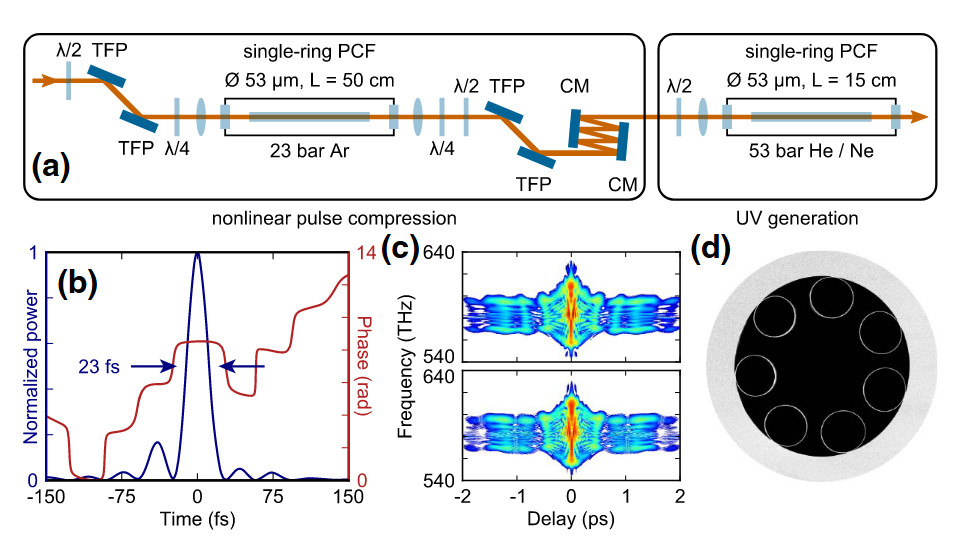
\includegraphics[width=0.6\textwidth]{p1.png}
    \caption{(a) 实验设置.  (b) 第二根光纤输入端在 100 kHz 重复频率下的时间脉冲形状. 在非线性压缩阶段之后, 通过二次谐波生成 FROG 测量脉冲. 随后的光学元件的色散以数字方式添加.  (c) 测量的 (顶部) 和检索的 (底部) FROG 迹线. 色阶覆盖 30 dB.  (d) 单环 PCF 的扫描电镜照片. }\label{p1}
\end{figure}

非线性压缩阶段: 首先通过自相位调制展宽光谱, 然后用负啁啾镜压缩. 

· 光谱展宽: 50 cm 长的 SR-PCF, 芯直径 53 $\mathrm{\mu m}$, 毛细管壁厚为 350 nm, 充 23 bar Ar. 

· 输入脉冲为圆偏振, 有效克尔非线性降低为线偏时的 2/3. 

· 压缩器设计为在 $\sim$ 20 $\mathrm{\mu J}$ 输入能量下工作. 

如此, 对给定输入能量, 可使用更高气压, 产生更弱反常色散和更高质量压缩脉冲. 经光纤后, 偏振转回线偏. 负啁啾反射镜 (UltraFast Innovations GmbH) 引入了 -2100 $\mathrm{fs^2}$ 的GDD, 以补偿光纤中自相位调制引起的正啁啾以及直至第二根光纤输入的光学器件色散. 

在非线性压缩阶段之后, 使用频率分辨光门控 (FROG) 以 100 kHz 重复频率测量脉冲 [图\ref{p1}(b) 和 (c)]或在每个重复频率下使用商用自相关器. 测量的自相关性不会随重复频率发生显着变化, 并且与通过 FROG 在 100 kHz 测量的脉冲计算出的结果非常一致. 

· 100 kHz - 1.92 MHz 重复频率下, 持续时间为 $\sim$ 300 fs 的 $\sim$ 20 $\mathrm{\mu J}$ 脉冲被压缩至 <25 fs [半高全宽 (FWHM)]

· 通过压缩器的传输率超 82\% (包括所有光学器件) . 

· 在最高重复频率下, 能量为 20.5 $\mathrm{\mu J}$ (平均功率为 39.3 W) 的脉冲被压缩至 $\sim$ 24 fs、17.4 $\mathrm{\mu J}$ (33.5 W) , 传输率为 85\%. 

· 结果实现了高效脉冲压缩, 在充气 SR-PCF 中, 非线性过程产生的新光谱分量保留了圆偏振, 长度超过 50 厘米, 具有高峰值和平均功率. 


\section{UV Generation}

\subsection{Experimental Setup for Second Stage}

第二阶段, 使用相同的 SR-PCF.

· 通过 HF 蚀刻处理将毛细管壁厚度减小至 $\sim$ 220 nm [SR-PCF 的蚀刻过程由 ultralumina 开发和执行 (\url{https://ultralumina.com})]. 这将 q=0 损耗带从 $\sim$ 740 nm 移至 470 nm, 减少其对脉冲动力学影响\cite{uebelBroadbandLightSource2020}. 原则上, 光纤可进一步蚀刻, 以实现从深紫外到近红外的无损耗带传输. 

· 二阶段输出用镀铝离轴抛物面镜 (Newport Corporation) 准直, 并通过氟化镁棱镜 (Korth Kristalle GmbH) 空间上分离紫外线. 棱镜被切割为以 200 nm 处的布鲁斯特角透射, 减小整个 UV 光谱区域内棱镜表面的菲涅耳损耗. 

· 用热功率计测量紫外功率, 并根据气体池窗口 (5 毫米厚的氟化镁, Thorlabs, Inc.) 的透射率和抛物面镜的反射率进行校正. 

· 使用光纤耦合CCD光谱仪来测量光谱. 

\subsection{Simulation for UV Generation}

为研究二阶段脉冲传播, 作者基于单向场方程进行数值模拟\cite{taniMultimodeUltrafastNonlinear2014}. 非线性由光学克尔效应 (使用文献\cite{lehmeierNonresonantThirdOrder1985}中的 $\chi_3$ 数据) 和光电离 (使用 Perelomov 等人的电离率\cite{perelomovIonizationAtomsAlternating1966}) 给出. 图 \ref{p2} 显示了一个示例. 

\begin{figure}[ht]
    \centering
    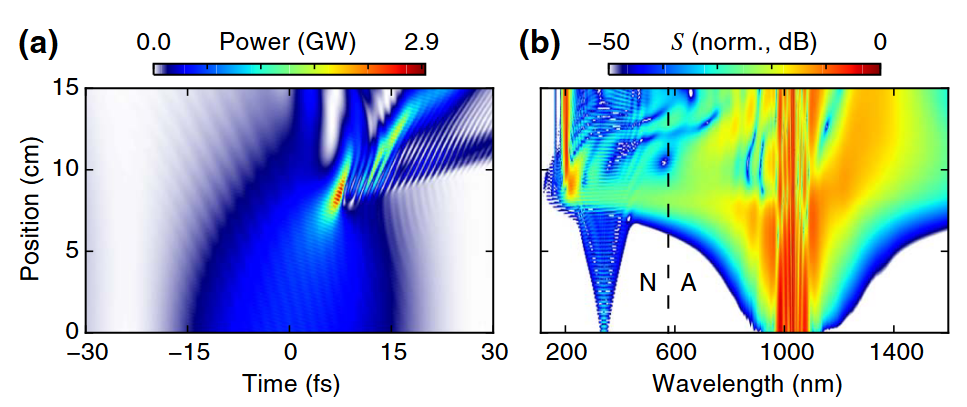
\includegraphics[width=0.6\textwidth]{p2.png}
    \caption{模拟 (a) 时域 (b) 频域脉冲在 SR-PCF 中的传播, 芯直径为 53 $\mathrm{\mu m}$, 填充有 53 bar He. 输入脉冲数据采用之前测量结果[图\ref{p1}(b)] 输入能量 17 $\mathrm{\mu J}$. S: 光谱能量密度. 零色散波长 (虚线) 位于 576 nm.  N 和 A 分别表示正常色散和反常色散区域. 输入脉冲自压缩至 1.1 fs FWHM 的持续时间, 然后发射 $\sim$ 200 nm 的 DW, 能量 2 $\mathrm{\mu J}$, 峰值功率达 0.3 GW.  DW 发射持续时间 <10 fs, 并在光纤输出处延长至 21 fs (这可通过优化光纤长度避免) }\label{p2}
\end{figure}

调整气压以实现反常色散, 泵浦脉冲会经历孤子动力学. 在足够高输入能量下, 最初脉冲会时域压缩并展宽光谱, 正如高阶孤子的预期. 

实验中, 孤子阶数低于 $\sim$ 6, 从而产生相干动力学. 随着脉冲压缩, 高阶效应开始发挥作用. 脉冲后缘的自陡峭和光学冲击效应导致强烈不对称的向较短波长方向的光谱展宽. 

深紫外中与 DW 的相位匹配是通过高阶色散实现的, 且在
\begin{equation}
    \beta(\omega_{\mathrm{DW}})=\beta_{\mathrm{sol}}(\omega_{\mathrm{DW}})
    \label{eq:2}
\end{equation}
时满足匹配条件, 其中 $\omega _{DW}$ 是 DW 频率, $\beta$ 和 $\beta_{\mathrm{sol}}$ 是线性波和孤子的传播常数. 

当条件不完全满足时, 失相率为
\begin{equation}
    \vartheta(\omega)=\beta(\omega)-\{\beta_{0}+\beta_{1}[\omega-\omega_{\mathrm{sol}}]+\gamma P_{P}\omega/\omega_{\mathrm{sol}}\}
    \label{eq:3}
\end{equation}
, 其中 $\beta _0$ 是传播常数, $\beta_1$ 是孤子中心频率 $\omega _{\mathrm{sol}}$ 处的反群速度, $\gamma$ 是$\omega sol$ 处与气体相关的非线性光纤参数, $P_P$ 是孤子峰值功率. 

\begin{figure}[ht]
    \centering
    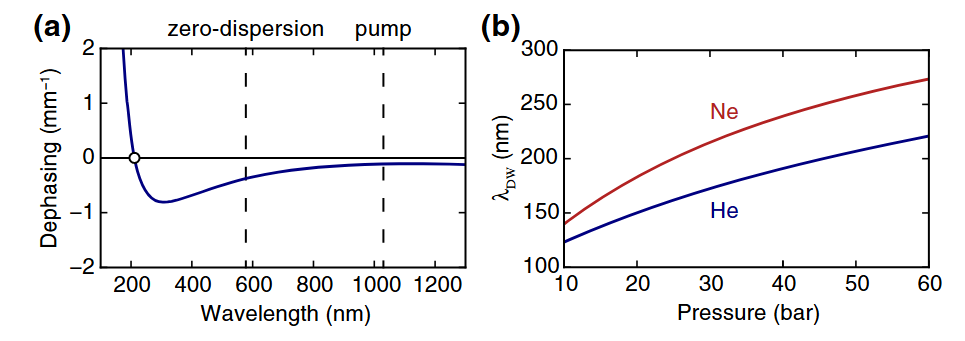
\includegraphics[width=0.6\textwidth]{p3.png}
    \caption{与 53 $\mathrm{\mu m}$ 纤芯直径的光纤和峰值功率 1 GW, 1030 nm 泵浦的 DW 进行相位匹配: (a) 填充有 53 bar He 的光纤的失相率 $\vartheta$. 相位匹配发生在 211 nm (圆点) 处. 充气光纤的微弱色散为宽带 DW 发射产生长的相干长度 (此处, 对于 15 nm/103 THz 的带宽, 相干长度超过 3 cm, 对应于 7.3\% 的相对带宽) .  (b) He 和 Ne 的相位匹配波长 $\lambda_{\mathrm{DW}}$ 与气压关系. }\label{p3}
\end{figure}

图 \ref{p3}(a) 绘制了给定一组光纤和气体参数的 $\vartheta$ 与波长的关系图.  

· DW 波长可通过核心直径、气体种类和压力进行广泛调节. 

· 增加气体压力或使用较重的气体会使相位匹配点红移, 而提高峰值功率会导致蓝移. 

· 泵浦脉冲在 DW 发射之前可能会经历大量蓝移 (通过电离) , 从而导致 DW 红移. 使用具有较高电离势的较轻气体, 通常可通过减少电离和更清洁的自压缩以及减少高重复频率效应 (稍后讨论) 来提高紫外线的转换效率. 

因此, 作者选择了最轻的气体, 可在目标波长下进行相位匹配 (高达气室的最大压力 - 60 bar) . 

\subsection{Result for Second Stage}

第二根光纤中充 He 和 Ne, 分别在 $\sim$ 200 和 $\sim$ 270 nm 的深紫外区演示了 DW 发射. 

\begin{figure}[ht]
    \centering
    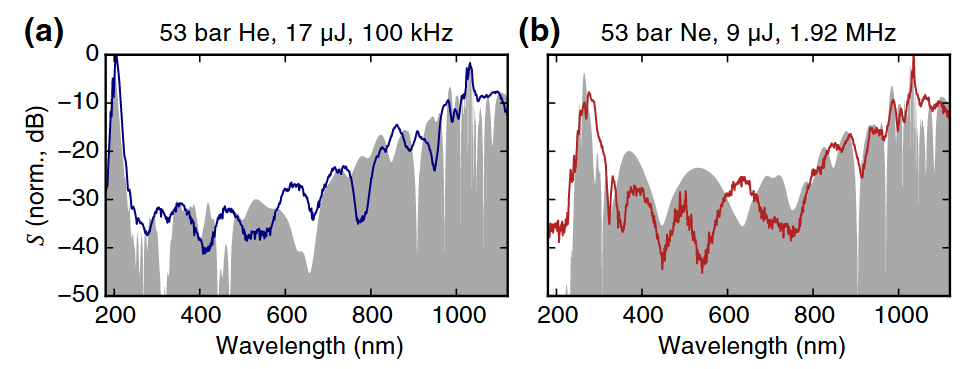
\includegraphics[width=0.6\textwidth]{p4.png}
    \caption{(a) 充 He, 以 100 kHz 重复频率泵浦 17 $\mathrm{\mu J}$ 脉冲, 测量 (蓝色) 和模拟 (灰色下阴影) 的光谱. 测得的 UV 脉冲能量为 1.05 $\mathrm{\mu J}$ (平均功率 105 mW) .  (b) 充Ne, 用 1.92 MHz 的 9 $\mathrm{\mu J}$ 脉冲泵浦, 测量 (红色) 和模拟 (灰色) 的光谱. 测得的 UV 脉冲能量为 0.54 $\mathrm{\mu J}$ (平均功率 1.03 W) . }\label{p4}
\end{figure}

图 \ref{p4} 实验测得 DW 生成 UV 光谱, (a) :

· 与相应模拟结果 (图\ref{p2}) 非常吻合;

· 光纤: He, 53 bar;

· 泵浦: 重复频率 100 kHz, 能量 17 $\mathrm{\mu J}$. 

· 发射 DW: 205 nm 波长, 1.05 $\mathrm{\mu J}$ 能量 (输入光纤能量的 6.2\% ), 对应 105 mW 的平均功率.  

· UV 光束轮廓保持为干净的基模, 

· DW 光谱表现出宽带宽 (7.9 nm/56 THz FWHM) , 支持 3.8 fs 的脉冲变换极限. 

先前已经表明, 充气 HC-PCF 中自压缩孤子发射的 DW 是超短的 (在 Ermolov 等人的工作中低于 5 fs\cite{ermolovCharacterizationFewfsDeepUV2016}) , 这一结果通过本文模拟得到证实. 对较长波长的 DW 发射, \ref{p4}(b):

· 53 bar Ne. 

· 泵浦: 100 kHz, 9 $\mathrm{\mu J}$

· DW发射: 264 nm, 能量 0.74 $\mathrm{\mu J}$ (光纤输入能量的 8.2\%) , 对应 74 mW 平均功率. 

\subsection{Repetition Rate Scaling}

10-20 $\mathrm{\mu J}$ 的适度的泵浦脉冲能量可允许 MHz 量级的重复频率 (当前实验中高达 1.92 MHz) , 但平均功率仅数十瓦. 结果如图 \ref{p5} 所示. 

\begin{figure}[ht]
    \centering
    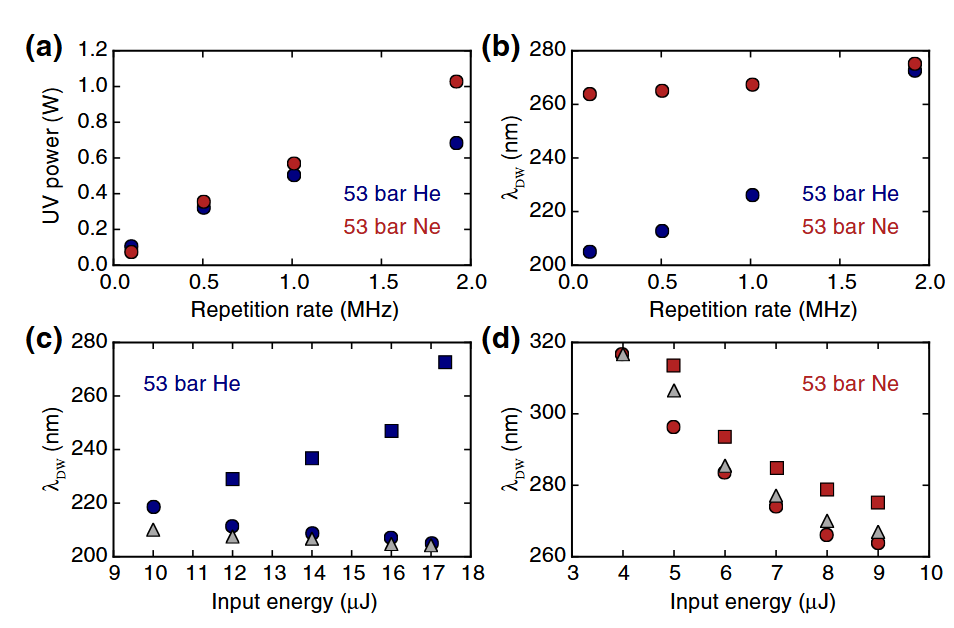
\includegraphics[width=0.6\textwidth]{p5.png}
    \caption{当光纤填充氦气和氖气时, (a) UV 区域功率和 (b) DW 波长 (光谱质心) 与重复频率的函数关系.  DW 波长作为光纤的输入能量的函数: (c) 充 He 和 (d) 充 Ne , 重复频率为 100 kHz (圆点) 和 1.92 MHz (方块) . 灰三角代表模拟. }\label{p5}
\end{figure}

· 虽紫外范围的平均功率随着重复频率的增加而增加, 但脉冲能量下降. 

· 尽管如此, 在 275 nm 处可获得 1.03 W 的平均功率 (光纤充氖, 1.92 MHz 重复频率) . 相应的光谱如图 \ref{p5} (b)所示. UV 中的脉冲能量仍有 0.54 $\mathrm{\mu J}$, 光纤输入能量的 6\% 转换为 UV. 

\section{Discussion}

随泵浦能量增加, DW 发射带通常向短波移动. 这是因为自压缩脉冲具更高峰值功率, 增强了克尔效应对失相参数 $\vartheta$ 的贡献. 

· 在充氖光纤中所有重复频率下都观察到了这种行为;

· 但在充氦光纤中的仅最低重复频率 (100 kHz) 下观察到了这种行为. 相反, 在 505 kHz 和 1.01 MHz 时, DW 最初随着输入能量增加而蓝移, 但随后随着输入能量进一步增加而红移. 在最高重复频率 (1.92 MHz) 下, 随着输入能量的增加, DW 不断向更长的波长移动, 在最高输入能量下达到 273 nm, 即 100 kHz 重复频率下的发射波长为 68 nm/363 THz [图\ref{p5}(c)]. 

· 在充氖光纤中观察到 DW 波长的重复频率依赖性要小得多, 当重复频率从 100 kHz 增加到 1.92 MHz 时, 红移仅为 11 nm/47 THz (264 至 275 nm) [图 \ref{p5} (b)]. 尽管这种随着重复频率增加而产生的红移可以通过降低气压来部分补偿, 但这是以降低紫外光转换效率为代价的. 

作者估计, 连续激光照射过程中等离子体积累对实验参数的影响可以忽略不计. 在任何情况下, 恒定的背景等离子体密度都会使色散更加反常, 并导致 DW 的蓝移, 而不是观察到的红移. 

实验观察的红移归因于通过非线性吸收和电离加热引起的压力驱动的纤芯直径的小幅增加 (核心壁非常薄且机械塑性) . 过往在散装气体的成丝过程中观察到了相关的高重复频率效应\cite{chengEffectLongTimescale2013}, 其演变时间尺度从纳秒到毫秒. 虽然它们尚未包含在已建立的光纤脉冲传播模型中, 但作者预计, 当系统在连续激光发射之间未完全恢复时, 它们尤其会在高重复频率下发生. 当 DW 发射波长较短时, 低重复频率 (100 kHz) 和高重复频率 (1.92 MHz) 之间的差异更加明显 [图 \ref{p5} (c)], 因为有效产生 DW 所需的强冲击效应会导致气体更强的电离 (根据模拟, 等离子体密度高达$3.1\times 10^{16}\; \mathrm{cm^{-3}}$, 电离引起的损失高达每个脉冲 16 nJ) . 然而, 如果将 DW 发射调谐到更长波长 [图  \ref{p5} (d)], 所需的泵脉冲压缩不太极端, 减少了电离 (等离子体密度高达 $1.6 \times  10^{15} \mathrm{cm^{-3}}$, 并且没有显着损失) , 并允许更好地重复频率缩放. 

为了进一步研究这一点，作者在光纤中填充不同气体，同时保持相似动力学，特别是 200 nm 左右的 DW 发射（图 \ref{p6}）。在 100 kHz 重复频率下，Kr 和 Ar 中的 UV 脉冲能量已在非常低的值处饱和，这与模拟相反。只有尽可能减少电离（使用氖和氦）才能在实验中产生高脉冲能量。剩余的差异可能是由于光纤损耗造成的，尽管此处也可以看到一些饱和度，但在模拟中忽略了光纤损耗。

\begin{figure}[h]
    \centering
    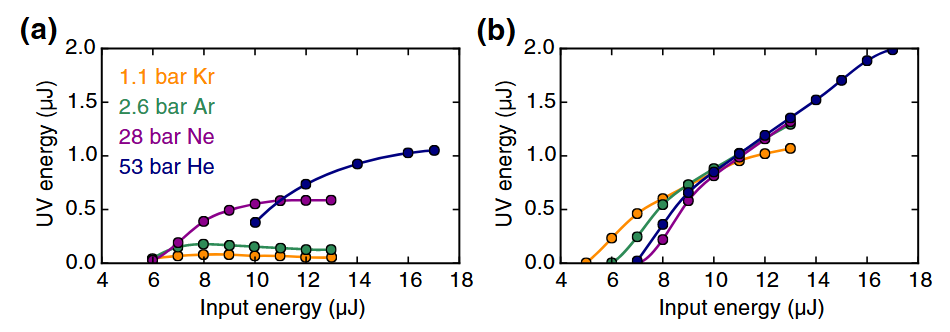
\includegraphics[width=0.6\textwidth]{p6.png}
    \caption{UV 脉冲能量: (a) 以 100 kHz 重复频率测量, (b) 模拟. 对每种气体, 调整压力以使 DW 发射波长为 $\sim$ 200-220 nm. 在模拟中, Kr 中电离损失高达 4.7 $\mathrm{\mu J}$, Ar 中电离损失高达 3.1 $\mathrm{\mu J}$, Ne 中电离损失高达 0.13 $\mathrm{\mu J}$, He 中电离损失高达 16 nJ. }\label{p6}
\end{figure}

进一步的实验表明，具有较小纤芯光纤对重复频率的依赖性更强。例如，在纤芯直径为 36 $\mathrm{\mu m}$ 的光纤中紫外光转换效率较低，且出现了高阶输出模式。

由于高重复频率下的动力学对许多 MHz 重复频率, 强场状态下运行的系统而言显然十分有趣，因此作者计划在未来实验中进一步研究。



%--------------------  插入参考文献  --------------------%

\newpage

\clearpage           %%%  “目录”中显示的页码正确, 需要添加 \clearpage
\phantomsection      %%   “目录”中的链接能正确跳转, 需要添加 \phantomsection
\addcontentsline{toc}{section}{参考文献}   %向目录中添加条目, 以章的名义

\bibliography{ref}

\end{document}